% Copyright(C) 2011-2015 Pedro H. Penna <pedrohenriquepenna@gmail.com>
%
% This file is part of Nanvix.
%
% Nanvix is free software; you can redistribute it and/or modify
% it under the terms of the GNU General Public License as published by
% the Free Software Foundation; either version 3 of the License, or
% (at your option) any later version.
%
% Nanvix is distributed in the hope that it will be useful,
% but WITHOUT ANY WARRANTY; without even the implied warranty of
% MERCHANTABILITY or FITNESS FOR A PARTICULAR PURPOSE. See the
% GNU General Public License for more details.
%
% You should have received a copy of the GNU General Public License
% along with Nanvix. If not, see <http://www.gnu.org/licenses/>.

\documentclass[10pt,a4paper]{article}

% Input.
\usepackage[utf8]{inputenc}
\usepackage[english]{babel}

% Figures.
\usepackage{graphicx}

% References.
\usepackage[backend=biber]{biblatex}

\author{Pedro H. Penna}
\title{The Nanvix Operating System}

\begin{document}

\maketitle

\section{Introduction}
\label{section: introduction}

% About Nanvix.
Nanvix is an operating system created by Pedro H. Penna for educational purposes. It was designed from scratch to be small and simple, and yet modern and fully featured, so that it could help both, novices and experienced enthusiasts in operating systems, to learn about kernel hacking. The first release of Nanvix came out in early 2011, and since then the system has gone through several changes. This paper details the internals of Nanvix 1.2. All previous and future releases are available at \url{github.com/ppenna/nanvix}, under the GPLv3 license.

% Paper organization.
In this section, we present an overview of Nanvix, starting with the system architecture, then presenting the system services, and finally discussing the required hardware to run the system. In later sections, we present a more detailed description of the system.

\subsection{System Architecture}
\label{section: system architecture}

% Nanvix and System V.
The architecture of Nanvix is outlined in Figure \ref{figure: nanvix architecture}. It presents a similar structure to Unix System V, and it has been intentionally designed to be so due to two points. First, several successful operating systems, such as Aix, Linux and Solaris, are based on this architecture. Second, System V has earned Dennis Ritchie and Kenneth Thompson the 1983 Turing Award. These points indicate that System V is a well-architected and reliable system, thus being a good baseline for a new educational operating system, such as Nanvix.

% Architecture overview.
Nanvix is structured in two layers. The kernel, the bottom layer, seats on the top of the hardware and runs in privileged mode, with full access to all resources. Its job is to extended the underlying hardware so that: (i) a more pleasant interface, which is easier to program, is exported to the higher level; and (ii) resources can be shared among users, fairly and concurrently. The userland, the higher layer, is where all user software (programs) run in unprivileged mode, with limited access to the hardware, and the place where the user itself interacts with the system.

% Kernel architecture.
The kernel presents a monolithic architecture, and it is structured in four subsystems: the hardware abstraction layer; the memory management system; the process management system; and the file system. The hardware abstraction layer interacts directly with the hardware and exports to the other subsystems a set of well defined low-level routines, such as those for dealing with IO devices, context switching and interrupt handling. Its job is to isolate, as much as possible, hardware intricacies, so that the kernel can be easily ported to other compatible platforms, by simply replacing the hardware abstraction layer.

\begin{figure}[t]
	\centering
	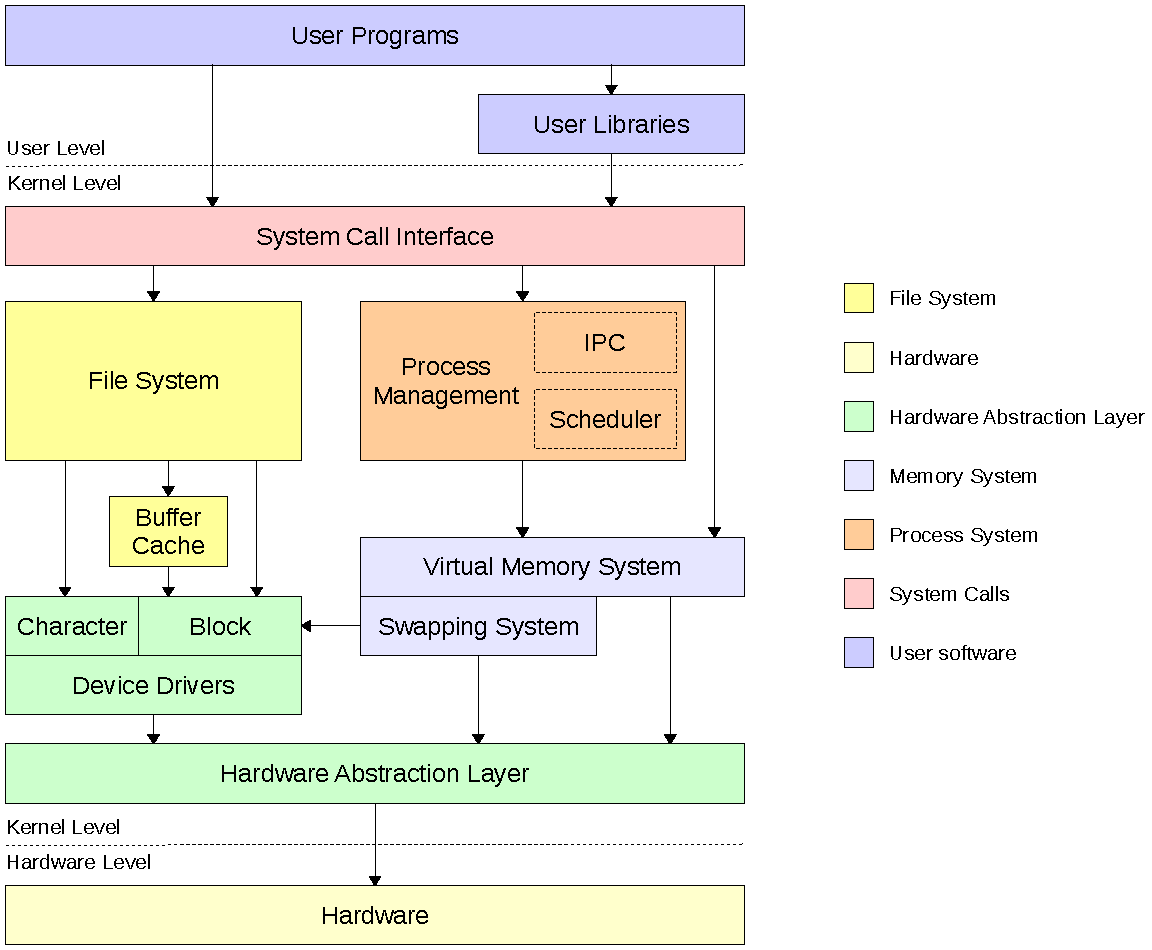
\includegraphics[scale=0.61]{img/nanvix-architecture}
	\caption{Nanvix architecture.}
	\label{figure: nanvix architecture}
\end{figure}

% Memory management system.
The memory management subsystem provides a flat virtual memory abstraction to the system. It does so by having two modules working together: the swapping and virtual memory modules. The swapping module deals with paging, keeping in memory those pages that are more frequently used, and swapping out to disk those that are not. The virtual memory system, on the other hand, relies on the paging module to manage higher-level abstractions called memory regions, and thus enable advanced features such as shared memory regions, on-demand loading, lazy coping and memory pinning.

% Process management system.
The process management system handles creation, destruction, scheduling, synchronization and communication of processes. Processes are single thread entities and are created on demand, either by the system itself or the user. Scheduling is based on preemption and happens in userland whenever a process runs out of quantum or blocks awaiting for a resource. In kernel land, on the other hand, processes run in nonpreemptive mode and scheduling occurs only when a processes voluntarily relinquishes the processor. Finally, processes many synchronize their activities using semaphores, and communicate with one another through pipes and shared memory regions.

% File system.
The file system provides a uniform interface for dealing with resources. It extends the device driver interface and creates on top of it the file abstraction. Files can be accessed through a unique pathname, and may be shared among several processes transparently.   The file system is compatible with the one present in the Minix 1 operating system, it adopts an hierarchical inode structure, and supports mounting points and disk block caching.

\subsection{System Services}
\label{section: system services}

\subsection{Hardware Requirements}
\label{section: hardware requirements}

\end{document}